\subsection{Dados e Análise
Descritiva.}\label{dados-e-analise-descritiva.}

Os dados são de peridiocidade diária, são disponibilizados pela
\href{http://www.cepea.esalq.usp.br/br/consultas-ao-banco-de-dados-do-site.aspx}{CEPEA/EXALQ}
e se referem ao período de 25/01/2010 a 20/01/2017, porém ao se
deflacionarem os dados a série foi reduzida para 29/12/2016 pois não
foram encontrados o índice de preço para o no de 2017. Os dados para o
etanol correspondem ao Indicador Diário do Etanol Hidratado
ESALQ/BM\&FBovespa Posto Paulínia (SP). Para o açúcar os dados são o
Indicador Açúcar Criatal CEPEA/EXALQ - São Paulo por saca de 50 quilos.
Para o soja os dados são o Indicador Soja CEPEA/EXALQ - Paraná por saca
de 60 quilos. Ocorreram 15 valores faltante para o soja durante o
período, estes dados foram interpolados pelo método \emph{spline}
conforme indicado por Zeileis and Grothendieck (2005).

\begin{longtable}[t]{lllll}
\caption{\label{tab:unnamed-chunk-5}Resumo das séries de preços}\\
\toprule
  &     acucar &     etanol &      soja &      Data\\
\midrule
 & Min.   :32.97 & Min.   : 732.5 & Min.   : 39.99 & Min.   :2010-01-25\\
 & 1st Qu.:48.25 & 1st Qu.:1105.1 & 1st Qu.: 49.13 & 1st Qu.:2011-10-20\\
 & Median :63.17 & Median :1190.5 & Median : 53.92 & Median :2013-07-24\\
 & Mean   :61.47 & Mean   :1238.0 & Mean   : 59.97 & Mean   :2013-07-23\\
 & 3rd Qu.:73.06 & 3rd Qu.:1317.0 & 3rd Qu.: 71.58 & 3rd Qu.:2015-04-23\\
 & Max.   :93.18 & Max.   :1924.5 & Max.   :100.92 & Max.   :2017-01-20\\
\bottomrule
\end{longtable}

Para vizualização dos dados foi plotado na
\protect\hyperlink{figura1}{Figura 1} os gráficos do logarítimo da série
de preços e do logarítimo da série de preços deflacionada. Os dados
foram deflacionados pelo Índice de Preço ao Produtor (IPP). Optou-se
pela apresentação na forma de logarítmo devido a diferença de escala
entre o preço do etanol e dos preços da soja e açúcar, além de que,
conforme Tsay (2012) as variáveis em logarítimo quando diferenciadas nos
dão uma aproximação da taxa de crescimento, ou no caso do mercado
financeiro, do retorno do ativo. A Figura 2 mostra a volatilidade medida
por \(v_i^2\) do etanol, açúcar e soja, sendo \(v_{i,t}\) uma medida
classificada na literatura de finanças como retorno do ativo e em outros
trabalhos como uma outra medida de volatilidade, sendo que:

\begin{equation}
v_{i,t} =\Delta \log p_{i,t}.
\end{equation}

Em que \(p_{i,t}\) é o preço da \emph{commodity} \(i\), \(t\) é o
período (dia, neste caso) e \(i = commodity \text{ de interesse}\).
Percebe-se que a volatilidade do preço do açúcar é bem mais intensa e
com maior amplitude se comparadas às volatilidades do preço do soja e do
preço do etanol. Entretanto, conforme López Cabrera and Schulz (2016) é
característico das séries de preços de \emph{commodities} serem
cointegradas e uma medida de volatilidade que leve em conta esta
característica dos dados se torna mais apropriada. Para isso pode-se
modelar a média da série de preços por meio de um modelo de correção de
erros (VECM, sigla em inglês) e então filtrar a série de preços do
co-movimento de suas médias condicionais. A partir de então podem ser
obtidas medidas de volatilidade livres da influência deste co-movimento
entre as médias condicionais de preços.

\begin{figure}[htbp]
\centering
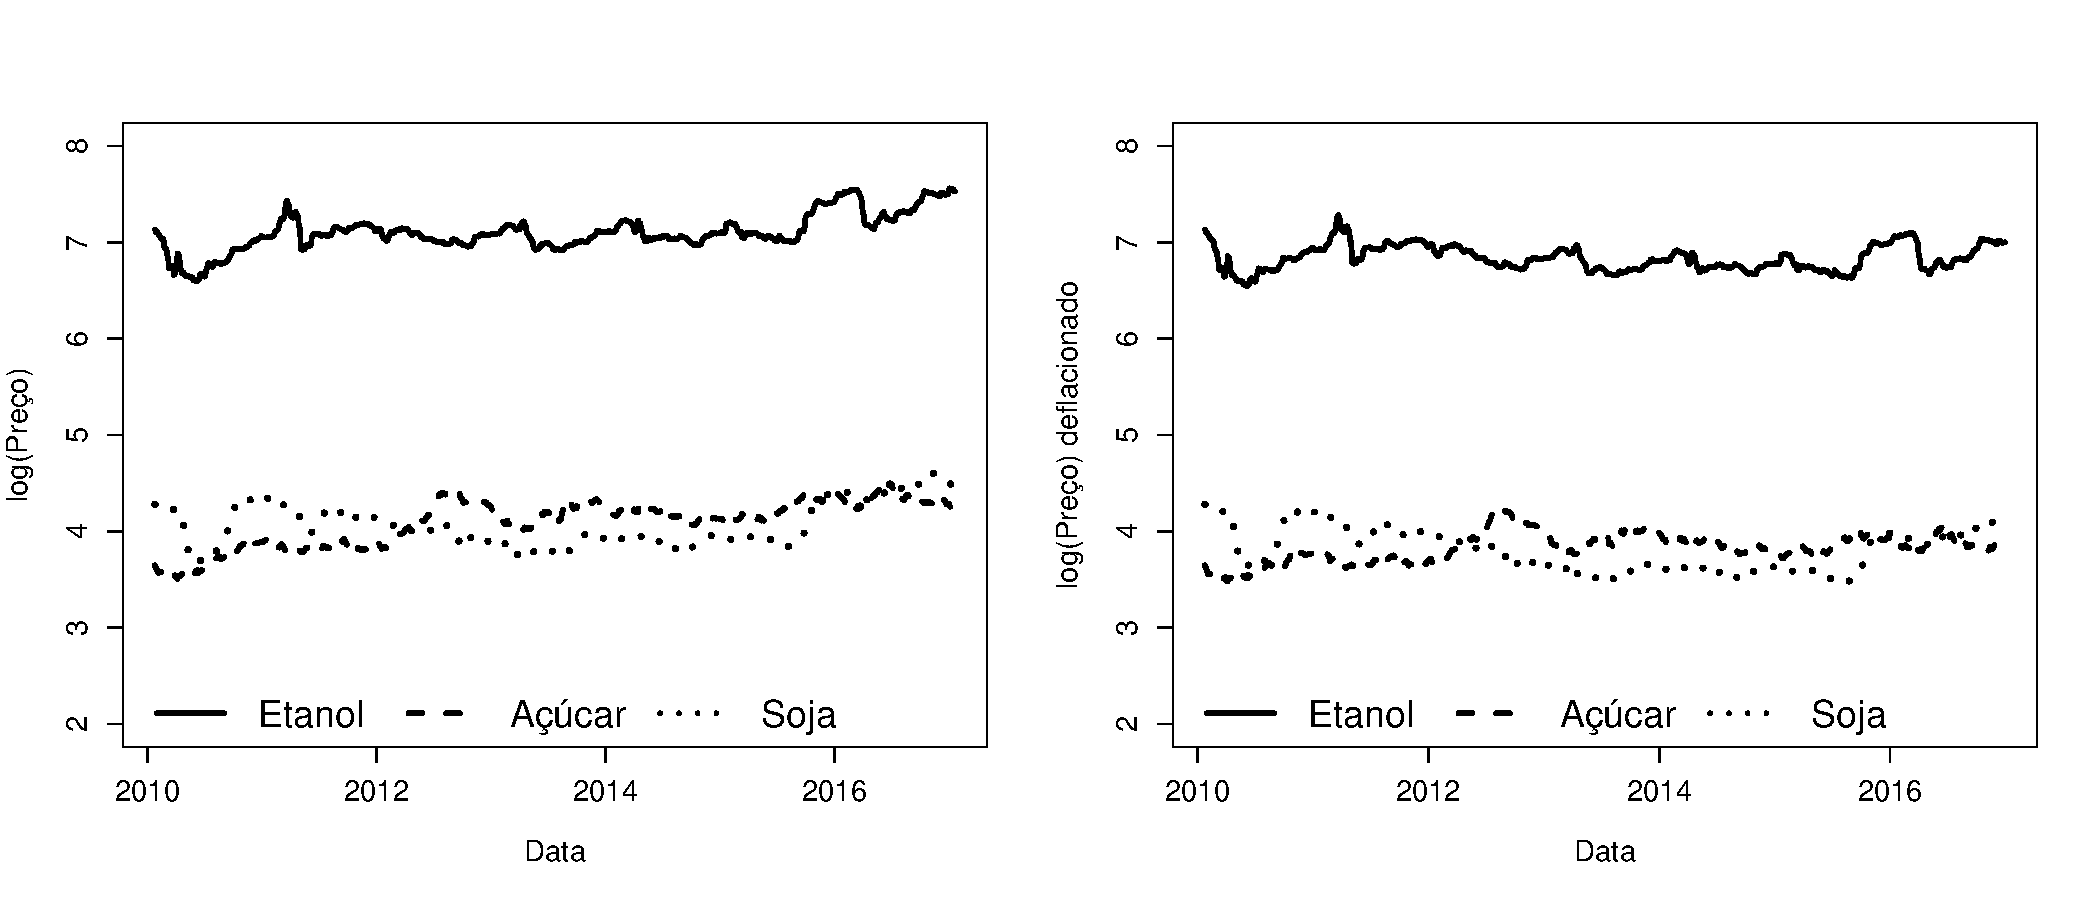
\includegraphics{dados_cepea_files/figure-latex/grafico1-1.pdf}
\caption{Logarítimo dos preços diários e preço diário deflacionado pelo
Ìndice de Preço do Produtor (IPP) para o etanol, açúcar e soja}
\end{figure}

\begin{figure}[htbp]
\centering
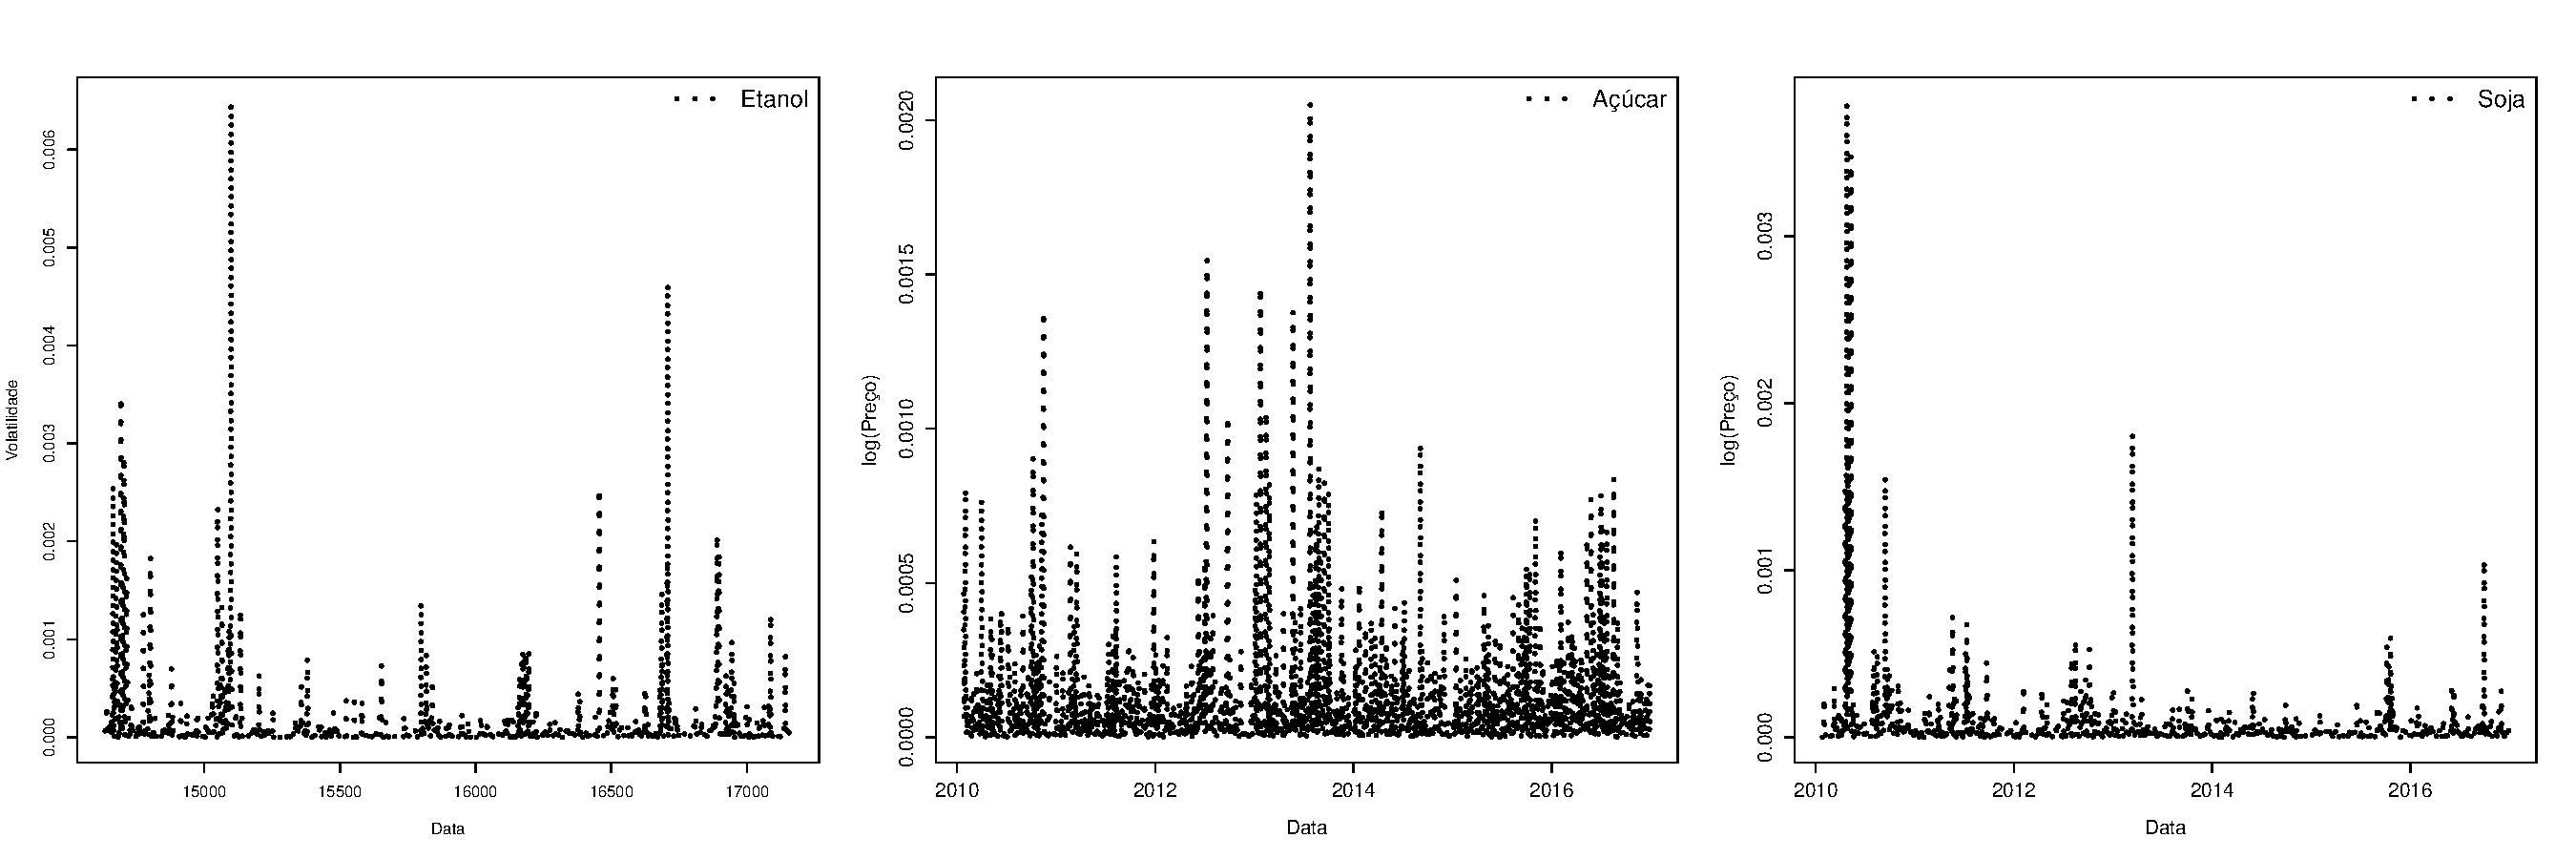
\includegraphics{dados_cepea_files/figure-latex/grafico2-1.pdf}
\caption{Volatilidade medida pela diferença do logarítimo do preço ao
quadrado para a etanol, açúcar e soja}
\end{figure}

\pagebreak

\begin{longtable}[]{@{}lrrr@{}}
\caption{Distribuição das variáveis.}\tabularnewline
\toprule
& Etanol & Açúcar & Soja\tabularnewline
\midrule
\endfirsthead
\toprule
& Etanol & Açúcar & Soja\tabularnewline
\midrule
\endhead
Média & 938,48 & 46,35 & 45,82\tabularnewline
Desvio Padrão & 126,37 & 6,82 & 10,64\tabularnewline
& & &\tabularnewline
Correlação & 1,00 & -0,22 & 0,60\tabularnewline
& & 1,00 & -0,41\tabularnewline
& & & 1,00\tabularnewline
Assimetria & -0,29 & -0,16 & -0,06\tabularnewline
Curtose & 12,33 & 4,29 & 12,85\tabularnewline
\(Q\)(20) & \textless{}0,01 & \textless{}0,01 &
\textless{}0,01\tabularnewline
\(Q^2\)(20) & \textless{}0.01 & \textless{}0,01 &
\textless{}0,01\tabularnewline
Arch & \textless{}0,01 & \textless{}0,01 &
\textless{}0,01\tabularnewline
Shapiro-Wilk & \textless{}0,01 & \textless{}0,01 &
\textless{}0,01\tabularnewline
\bottomrule
\end{longtable}

Na Tabela 2 são apresentados a média, desvio padrão e correlações do
nível de preços do etanol, açúcar e soja. O preço do açúcar é
positovamente correlacionado com o preço do etanol, o que era de se
esperar pois os dois produtos são substitutos na perspectiva do
produtor. Por exemplo, caso o preço do etanol esteja elevado e apresente
maior lucratividade em relação ao açúcar, o produtor tende a aumentar a
oferta de etanol e reduzir a oferta de açúcar, o que por sua vez,
aumenta o preço do açúcar. A correlação entre soja e etanol é positiva.
Esta tendência explica os co-movimentos dos preços das
\emph{commodities} no mercado financeiro internacional. Quanto à
correlação negativa entre o soja e o açúcar, a análise é mais indireta
em que tal correlação pode ocorrer devido a características espculativas
inerentes do mercado financeiro.

As outras estatísticas da Tabela 2 se referem à volatilidade,
\(v_{i,t}\). As três séries apresentam assimetria à esquerda em sua
distribuição. As volatilidades de soja e etanol apresentam elevado grau
de leptocurtose (12,33 e 12,85) enquanto o nível de leptocurtose do
açúcar (4,29) é bem inferior às outras duas \emph{commodities}. Para os
testes foram reportados o valor-p. \(Q\)(20) e \(Q^2\)(20) são os testes
de Ljung-Box para \(v_{i,t}\) e \(v_{i,t}^2\) respectivamente com 20
defasagens em ambos os testes, para mais detalhes sobre o teste consulte
McLeod and Li (1983). Os teste \(Q\) possui hipótese nula de ausência de
autocorrelação:

\begin{equation}
 H_0: \rho_1=\rho_2=\ldots=\rho_m=0
 \end{equation}

contra a ipótese alternativa de que pelo menos um coeficiente de
autocorrelação é diferente de zero:

\begin{equation}
H_a:\exists \;\rho_i\neq 0, \quad i =1,\ldots,m
\end{equation}

Conforme Tsay (2012), a regra de decisão é rejeitar a hipótese nula caso
o valor-p seja inferior ao nível de significância desejado. Os testes
tanto para a \(v_{it}\) quanto para \(v_{it}^2\) possuem valor-p
inferiores a 1\% o que nos leva a rejeitar a hipótese nula de ausência
de autocorrelação para as três séries e, com isso, as volatilidades não
são independentemente distribuídas. Arch é o teste de efeitos ARCH de
Engle (1982) que é um teste de multiplicador de Lagrange para
heterocedasticidade condicional. Este teste é equivalente à estatística
\(F\) para testarmod se \(\alpha_i=0\), \(i=1,\ldots,m\), na regressão
linear

\begin{equation}
a_t^2=\alpha_0+\alpha_1a_{t-1}^2+\ldots+\alpha_ma_{t-m}^2+\varepsilon_t,\quad t=m+1,\ldots,T.
\end{equation}

Em que \(a_t=v_t-\mu_t\), ou seja, o resíduo em relação à média
condicional, \(\varepsilon_t\) é o termo de erro, \(m\) é o número de
defasagens incluídas no teste e \(T\) o tamanho da amostra. A série ao
quadrado \(a_t^2\) é usada para checar a heterocedasticidade
condicional, cujo teste possui a hipótese nula

\begin{equation}
H_0:\alpha_1=\ldots=\alpha_m=0,
\end{equation}

contra a hipótese alternativa

\begin{equation}
H_a:\exists \; \alpha_i\neq 0, \quad i=1,\ldots,m.
\end{equation}

Maiores detalhes sobre o cálculo destas estatísticas também podem ser
encontrados em Tsay (2012). A regra de decião é rejeitar a hipótese nula
se o valor-p for menor que o nível de significânci desejado.Portanto, no
teste de efeito ARCH rejeitou-se a hipótese nula de ausência de
heterocedasticidade condicional para as três séries a um nível de
significância de 1\%. Com isso inferimos que existe heterocedasticidade
condicional nas séries estudadas.

Para testar a normalidade dos dados realizou-se o teste Shapiro-Wilk,
inicialmente desenvolvido por Shapiro and Wilk (1965). Este teste infere
se a amostra estudada veio de uma distribuição normal. Como os valores-p
reportados na Tabela 2 são menores que o nível de significância de 1\%,
rejeita-se a hipótese nula de que os dados foram amostrados de uma
distribuição normal. Até então todos as estatísticas estão em
conformidade com a literatura de volatilidade no mercado financeiro, em
que os dados apresentam leptocurtose, assimtetria à esquerda,
heterocedasticidade condicional e não normalidade em sua distribuição.
Alguns trabalhos recentes que identificaram estas características são,
López Cabrera and Schulz (2016), Freitas et al. (2015) e Araujo and
Montini (2015), para uma excelente revisão sobre o assunto, veja Serra
and Zilberman (2013).

\subsection{Testes de estacionariedade, raiz unitária e
cointegração.}\label{testes-de-estacionariedade-raiz-unitaria-e-cointegracao.}

Em seguida foram feitos os testes Dickey-Fuller aumentado (ADF, sigla em
inglês), KPSS e Phillips-Perron para identificar se as séries de preços
possuem raiz unitária, no caso dos testes ADF e Phillips-Perron ou se as
séries de preços são estacionárias, por meio do teste KPSS. A Tabela 3
mostra as estatísticas do teste KPSS e o valor tabela por nível de
significância. Podemos ver nesta tabela que todas as estatísticas,
independente da especificação do modelo, são maiores que os valores
tabelasdos, portanto não rejeitamos a hipótese nula de estacionariedade.
As tabelas 4 e 6 mostram os testes ADF e Phillips-Perron
respectivamente. A diferença destes dois testes em relação ao teste
KPSS, é que eles possuem hipótese nula de existência de raiz unitária.
Conforme as duas tabelas 4 e 6, para qualquer epecificação do modelo não
rejeitamos a hipótese nula de existência de raiz unitária nas séries
estudadas. Uma vez que evidenciamos a existência de raiz unitária nas
séries de preços, foram realizados os mesmos testes para as séries em
primeira diferença, onde constatou-se que elas são integradas em
primeira ordem. A partir disso podemos prosseguir para a identificação
de cointegração e estimação do modelo devetor de correção de erros
(VECM, sigla em inglês).

\begin{longtable}[t]{lrrrrrrr}
\caption{\label{tab:ADF e KPSS nivel}Teste KPSS preço em nível}\\
\toprule
  & etanol & acucar & soja & 1 Pct & 2.5 Pct & 5 Pct & 10 Pct\\
\midrule
Time Trend: & 1.57 & 3.80 & 5.17 & 0.22 & 0.18 & 0.15 & 0.12\\
No Trend: & 1.88 & 10.65 & 9.45 & 0.74 & 0.57 & 0.46 & 0.35\\
\bottomrule
\end{longtable}

\begin{longtable}[t]{lrrrrrrr}
\caption{\label{tab:ADF e KPSS nivel}Teste ADF preço em nível}\\
\toprule
  & etanol & acucar & soja & 1 Pct & 2.5 Pct & 5 Pct & 10 Pct\\
\midrule
Time Trend: & -3.83 & -1.67 & -2.44 & -3.96 & -3.66 & -3.41 & -3.12\\
Constant: & -3.87 & -1.90 & -2.67 & -3.43 & -3.12 & -2.86 & -2.57\\
Neither: & -0.16 & 0.27 & -0.39 & -2.58 & -2.23 & -1.95 & -1.62\\
\bottomrule
\end{longtable}

\begin{longtable}[t]{lrrr}
\caption{\label{tab:ADF e KPSS nivel}Defasagens do teste ADF}\\
\toprule
  & Trend Model & Drift Model & None\\
\midrule
etanol & 2 & 2 & 2\\
acucar & 1 & 1 & 1\\
soja & 6 & 6 & 5\\
\bottomrule
\end{longtable}

\begin{longtable}[]{@{}lrrr@{}}
\caption{Teste Phillips-Perron}\tabularnewline
\toprule
& Z(\(\alpha\)) & Defasagem & valor-p\tabularnewline
\midrule
\endfirsthead
\toprule
& Z(\(\alpha\)) & Defasagem & valor-p\tabularnewline
\midrule
\endhead
Etanol & -18,99 & 8 & 0,09\tabularnewline
Açúcar & -6,74 & 8 & 0,07\tabularnewline
Soja & -3,90 & 8 & 0,90\tabularnewline
\bottomrule
\end{longtable}

Como critério para seleção da ordem de defasagem do modelo VAR usamos os
critério AIC, BIC e HQ. Estes testes reportaram como número de
defasagens ótimas, 7, 4 e 6, respectivamente e por uma questão de
parcimômia usamos o número de defasagens sugerido pelo critério BIC (4
defasagens). Como o número ótimo de defasgens do modelo VAR é 4, para o
teste de cointegração devemos usar 3 defasagens. O teste realizado foi o
teste do traço de Johansen que possui hipótese nula de ausência de
cointegração contra uma hipótese alternativa de cointegração entre as
variáveis. O teste do traço verifica se o posto (\emph{rank}) da matriz
de cointegração \(\Pi = \alpha \beta'\) é igual a zero. a hipótese
alternativa é a de que \(0<rank(\Pi)<n\) e \(n\) é o número máximo
possível de vetores de cointegração. Se a hipótese nula de que o posto
da matriz \(\Pi\) seja zero for rejeitada, realiza-se o teste novamente
com a hipótese nula de que o posto seja 1 e assim sucessivamente até não
se rejeitar a hipótese nula. O posto da matriz \(\Pi\) será definido
logo quando não se rejeitar a hipótese nula do teste. O número de
vetores de cointegração é igual ao posto da matriz \(\Pi\).

\begin{longtable}[]{@{}llrr@{}}
\caption{Teste do traço de Johansen}\tabularnewline
\toprule
\(H_0\) & \(H_a\) & Estatística do teste & Valor crítico a
5\%\tabularnewline
\midrule
\endfirsthead
\toprule
\(H_0\) & \(H_a\) & Estatística do teste & Valor crítico a
5\%\tabularnewline
\midrule
\endhead
\(r=0\) & \(r>0\) & 42,16 & 31,52\tabularnewline
\(r\leq 1\) & \(r>1\) & 13,22 & 17,95\tabularnewline
\(r\leq 2\) & \(r>2\) & 4,12 & 8,18\tabularnewline
\bottomrule
\end{longtable}

Como se veerifica na Tabela 7, inicialmente rejeitou-se a hipótese nula
de que o posto da matriz \(\Pi\) seja zero, em seguida não se rejeitou a
hipótese nula de que o posto seja igual a um. Logo, exite uma única
relação de cointegração dada por:

\begin{equation}\label{coint}
p_t^e-0,03\,p_t^a-0,316\,p_t^s=0
\end{equation}

em que \(P_t^e\), \(p_t^a\) e \(p_t^s\) são os preços do etanol, açúcar
e soja, respectivamente. Agora, dado o vetor de cointegração, podemos
estimar o modelo VECM para obtermos a volatilidade livre do co-movimento
entre as médias dos preços.

\subsection{Estimação do modelo de vetor de correção de
erros.}\label{estimacao-do-modelo-de-vetor-de-correcao-de-erros.}

Foi estimado um modelo de vetor de correção de erros a partir do vetor
de cointegração encontrado anteriormen. Tanto a relação de longo prazo,
quanto a dinâmica de curto prazo são capturadas por este modelo. Depois
de realizado um refinamento ao remover os coeficientes não segnificantes
a \(5\%\) o modelo parcimonioso ficou (erro padrão entre parênteses):

\begin{align}\label{vecm}
\Delta p_t^e &=-\underset{(0,002)}{0,01}\hat{\beta}^Tp_{t-1}+\underset{(0,024)}{0,373}\Delta p_{t-1}^e+\underset{(0,024)}{0,258}\Delta p_{t-2}^e+\underset{(0,015)}{0,061}\Delta p^s_{t-2}+\underset{(0,024)}{0,036}\Delta p^e_{t-3}+u_t,\nonumber\\
\Delta p_t^a &=-\underset{(0,002)}{0,005}\hat{\beta}^Tp_{t-1}-\underset{(0,021)}{0,057}\Delta p^e_{t-1}+\underset{(0,023)}{0,2}\Delta p^a_{t-1}-\underset{(0,017)}{0,026}\Delta p_{t-2}^s-\underset{(0,022)}{0,043}\Delta p_{t-3}^e+u_t,\\
\Delta p_t^s &=\underset{(0,023)}{0,22}\Delta p_{t-1}^s+\underset{(0,024)}{0,174}\Delta p_{t-2}^s+\underset{(0,023)}{0,23}\Delta p_{t-3}^s+u_t.\nonumber
\end{align}

em que \(\hat{\beta}^Tp_{t-1}\) é a relação de cointegração estimada na
equação \eqref{coint}. Dado que os preços são diários o conjunto de
equações em \eqref{vecm} representam as mudanças percentuais de um dia
para o outro. Com relação ao etanol, a relação de longo prazo entre as
variáveis impacta negativamente o retorno do ativo (\(\Delta p_t\)). O
retorno do etanol sofre impacto de seus componentes autorregressivos e
do retorno do soja na dfasagem de segunda ordem, porém é um efeito fraco
se comparado com os componentes autorregresivos.

O retorno do açúcar também sofre impacto negativo dos co-movimento entre
as médias dos preços, assim como o retorno do etanol. Já seus
componentes autorregressivos impactam seu retorno de forma positiva, já
que o efeitoautorregressivo de primeira ordem sobrepõe o efeito de
terceira ordem. O etanom impacta o retorno do açúcar de forma negativa,
fato que corrobora a relação direta de oferta entre os dois produtos.
Para o açúcar, desta-se ainda um efeito significativo do soja no termo
de segunda defasafem, porém, como para o etanol, o efeito é muito fraco
e dissipado pelos componentes autorregressivos. Por fim o retorno do
soja também possui forte impacto positivo de seus componentes
autorregressvos e não apresenta nehuma influência significativa dos
demais retornos.

Na figura 3 estão plotados os resíduos do modelo VECM estimado com
refinamento. Visualmente fica perceptível a heterocedasticidade
condicional dos termos de erro, porém alguns teste estatísticos para
detectar a heterocedasticidade condicional ainda são nessários. Os
testes escolhidos foram os testes de Potmanteau e os teste baseados no
posto. Como consta na Tabela 8 os três primeiros testes se referem ao
teste de Portmanteau (\(Q^*_k(m)\) ) e suas extensões , a versão
ajustada para a média (\(Q^*(m)\) ) e a versão robusta com truncamento
de cauda superior de 5\% (\(Q^r_k(m)\)), e també o teste de posto
(\(Q_R(m)\)). Para mais detalhes sobre estes testes Tsay (2013) fornece
um excelente ponto de partida.

\begin{figure}[htbp]
\centering
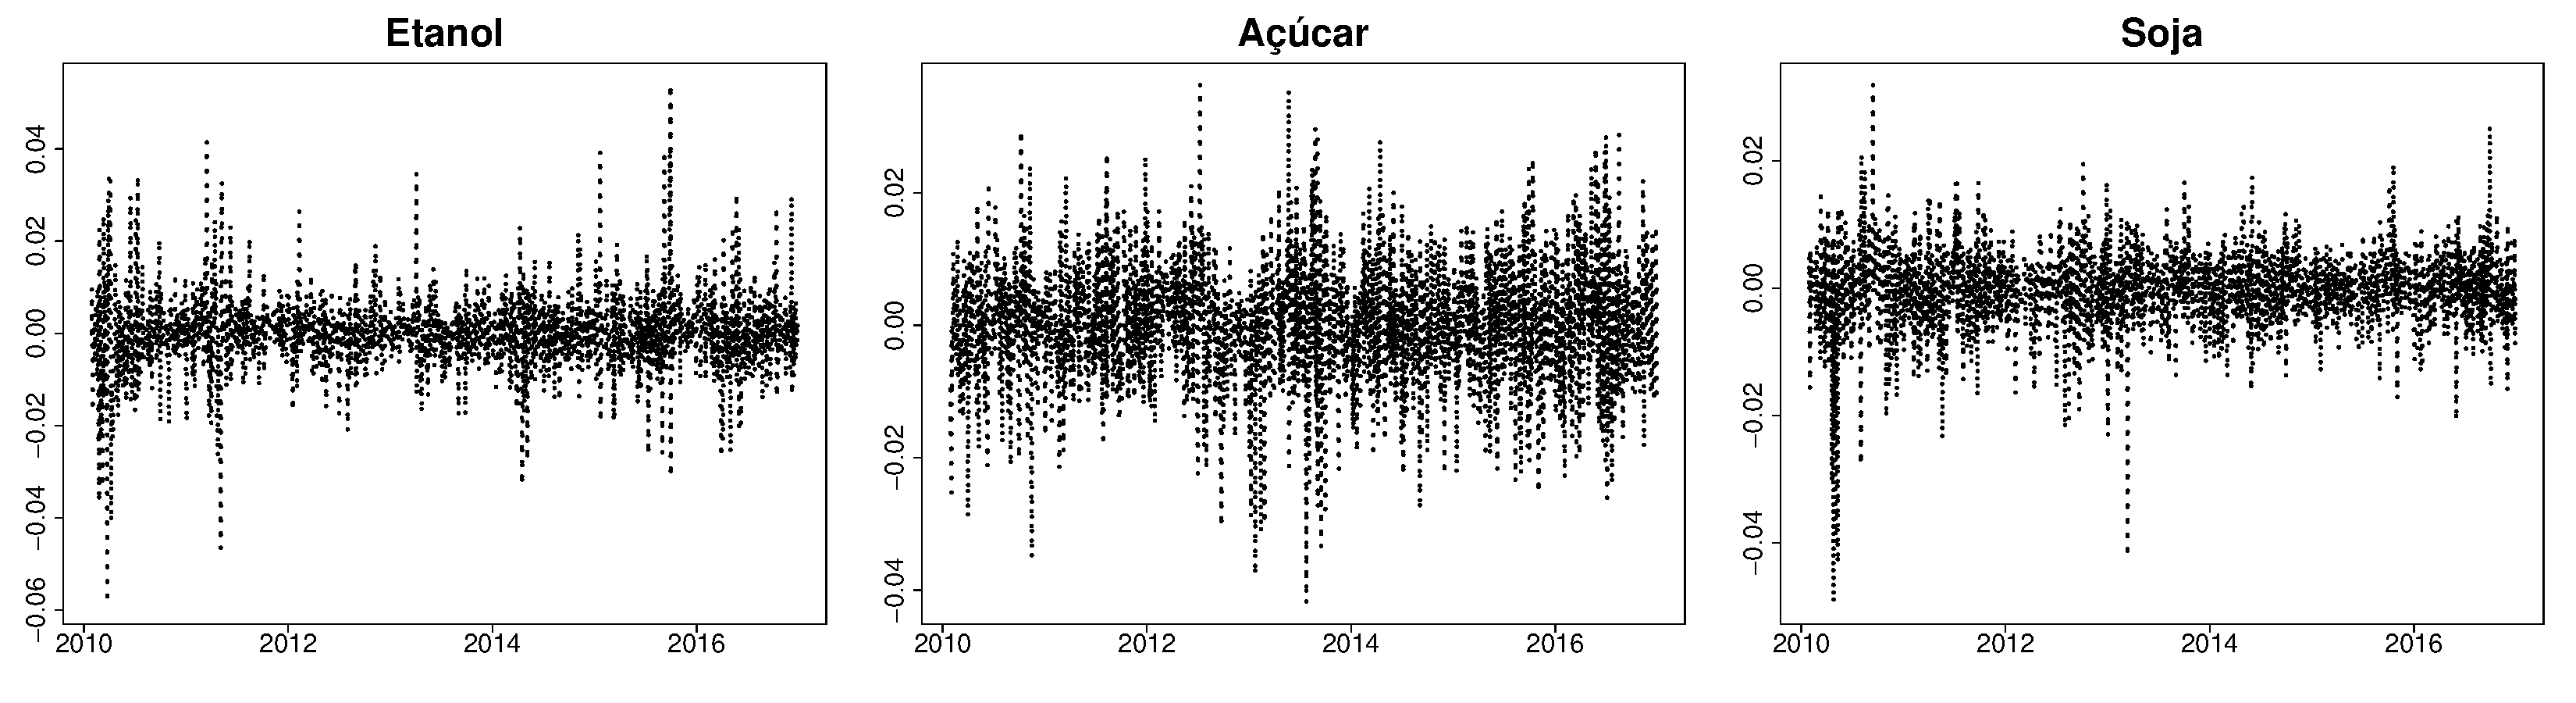
\includegraphics{dados_cepea_files/figure-latex/VECM resid-1.pdf}
\caption{Resíduos das estimação do modelo de vetor de correção de erros
(VECM)}
\end{figure}

\begin{longtable}[]{@{}lllll@{}}
\caption{Testes de heterocedasticidade condicional.}\tabularnewline
\toprule
& \(Q^*_k(m)\) & \(Q^*(m)\) & \(Q^r_k(m)\) & \(Q_R(m)\)\tabularnewline
\midrule
\endfirsthead
\toprule
& \(Q^*_k(m)\) & \(Q^*(m)\) & \(Q^r_k(m)\) & \(Q_R(m)\)\tabularnewline
\midrule
\endhead
Teste & 646,09 & 213,39 & 503,87 & 184,77\tabularnewline
valor-p & \textless{}0,01 & \textless{}0,01 & \textless{}0,01 &
\textless{}0,01\tabularnewline
\bottomrule
\end{longtable}

Todos os teste falharam em rejeitar a hipótese nula de ausência de
heterocedasticidade condicional a um nível de significância inferior a
1\%, como era o esperado já que observamos na Figura 3 que os dados
sugeriam a ocorrência de heterocedasticidade condicional e os dados por
se tratarem de séries financeiras possuem este comportamento. Uma vez
que foi indentifaca a heterocedasticidade condicional para a série de
dados podemos modelar a heterocedasticidade condicional.

